\documentclass[conference]{IEEEtran}
\usepackage{times}

% numbers option provides compact numerical references in the text. 
\usepackage[numbers]{natbib}
\usepackage{multicol}
\usepackage[bookmarks=true]{hyperref}
\usepackage{float}
\usepackage{graphicx}
\graphicspath{ {images/} }

\pdfinfo{
   /Author (Ron Domingo)
   /Title  (Autonomous Driving: Safe Driving through Imitation Learning)
   /CreationDate (D:20101201120000)
   /Subject (Autonomous Driving)
   /Keywords (Autonomous Driving;CNN;Imitation Learning)
}

\begin{document}

% paper title
\title{Autonomous Driving: Safe Driving through Imitation Learning}

% You will get a Paper-ID when submitting a pdf file to the conference system
\author{\authorblockN{Ron Domingo}
\authorblockA{Department of Electrical Engineering\\
Stanford University\\
Email: rdomingo@stanford.edu}}


\maketitle

\begin{abstract}
The abstract goes here.
\end{abstract}

\IEEEpeerreviewmaketitle

\section{Introduction}
Path planning is a complex yet essential aspect of autonomous driving that is required
for vehicles to traverse the world around us. Finding paths is a complicated task that 
involves the avoidance of both static and dynamic obstacles, all while ensuring that the
vehicle stays within the drivable area of the road. \par
Imitation learning has become a popular method through which autonomous vehicles (AVs) are 
taught to handle the world around them. Given the complexity of the self-driving task,
traditional reinforcement learning for the self-driving problem has proven to become intractable
for the exponentially large state space associated with autonomous driving. Thus imitation learning
can significantly speed up the learning process for AVs by embedding some proper behavior within 
the learning process of the vehicle \cite{imitationLearning}. \par
This paper aims to apply imitation learning algorithms to teach an AV to drive around a closed loop
track while avoiding obstacles. The AV will be simulated using the Duckietown \cite{gym_duckietown} 
self-driving car simulator environments for OpenAI Gym. The goal of this paper is not only to
drive the simulated vehicle around Duckietown without colliding into obstacles but also to ensure
that the vehicle stays within the confines of the road surface, even when avoiding obstacles. \par
For the purposes of the project, general road rules will not be considered when driving
around the map and purely a drivable path around the road will be considered. 

\section{Related Works}


\section{Methods}

\subsection{Simulation Environment}
The Duckietown self-driving car simulator is an OpenAI Gym extension that serves as a 
simulator for the Duckietown hardware robots. The driving environment features marked roads, 
intersections, static objects such as buildings and trees, and finally dynamic obstacles 
like pedestrians that move around throughout the maps randomly. \par
\begin{figure}[H]
  \centering
    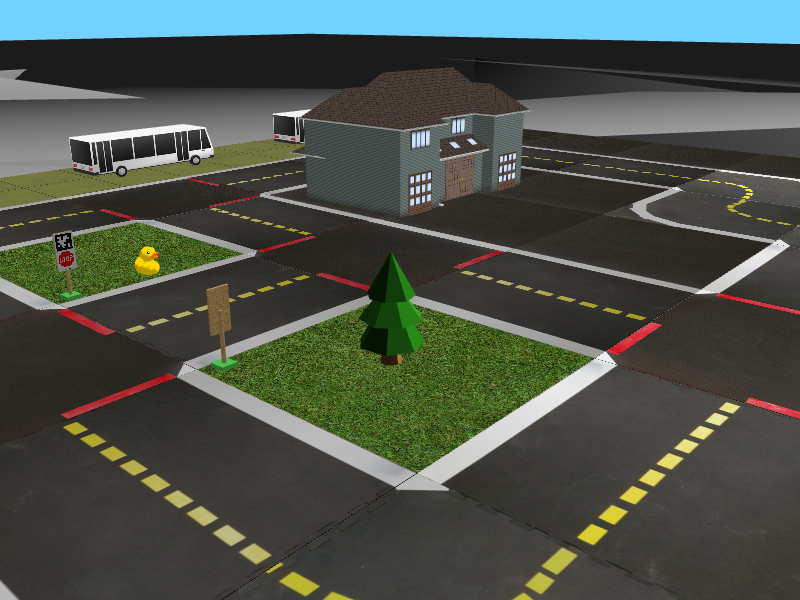
\includegraphics[scale=0.25]{simplesim_free.png}
  \caption{Simulation environment screenshot.}
\end{figure}
The Duckietown simulator outputs observations from a monocular camera mounted on the robot
with image sizes of 120x160x3. The vehicle takes in two parameters for each action, the velocity
and the steering angle.  \par 
Duckietown features customizable tracks ranging from mini-cities complete with intersections, signage,
pedestrians, and buildings, to simplified straight line tracks. For the purposes of this paper,
custom closed loop tracks are considered since the AV will be evaluated on its ability to maneuver 
around the track and get back to its original positition without colliding with any obstacles along 
the way. The tracks, however, will be customized so as to provide the AV with various training and 
test tracks for evaluation. Each track will also include a collection of randomly placed obstacles 
throughout, whether they are static of dynamic obstacles on or off the road surface. This is done 
to ensure that the AV can handle maneuvers such as stopping for pedestrians or swerving around static 
objects that lie in the road. Another purpose of this randomization is to prevent the AV from simply
memorizing the tracks and different maneuvers from the testing tracks. 

\subsection{Input Processing}
The Duckietown simulator provides observations in terms of images of size 120x160x3. In order to 
process these images, a Convolutional Neural Network is used to convert the raw images to the 
desired action (velocity, and steering angle).
The CNN architecture is as follows: 
\begin{itemize}
  \item Convolutional Block 
  \item Convolutional Block 
  \item Convolutional Block 
  \item Convolutional Block 
  \item Dropout
  \item Fully Connected Layer
  \item Fully Connected Layer
\end{itemize}
\begin{figure}[H]
  \centering
    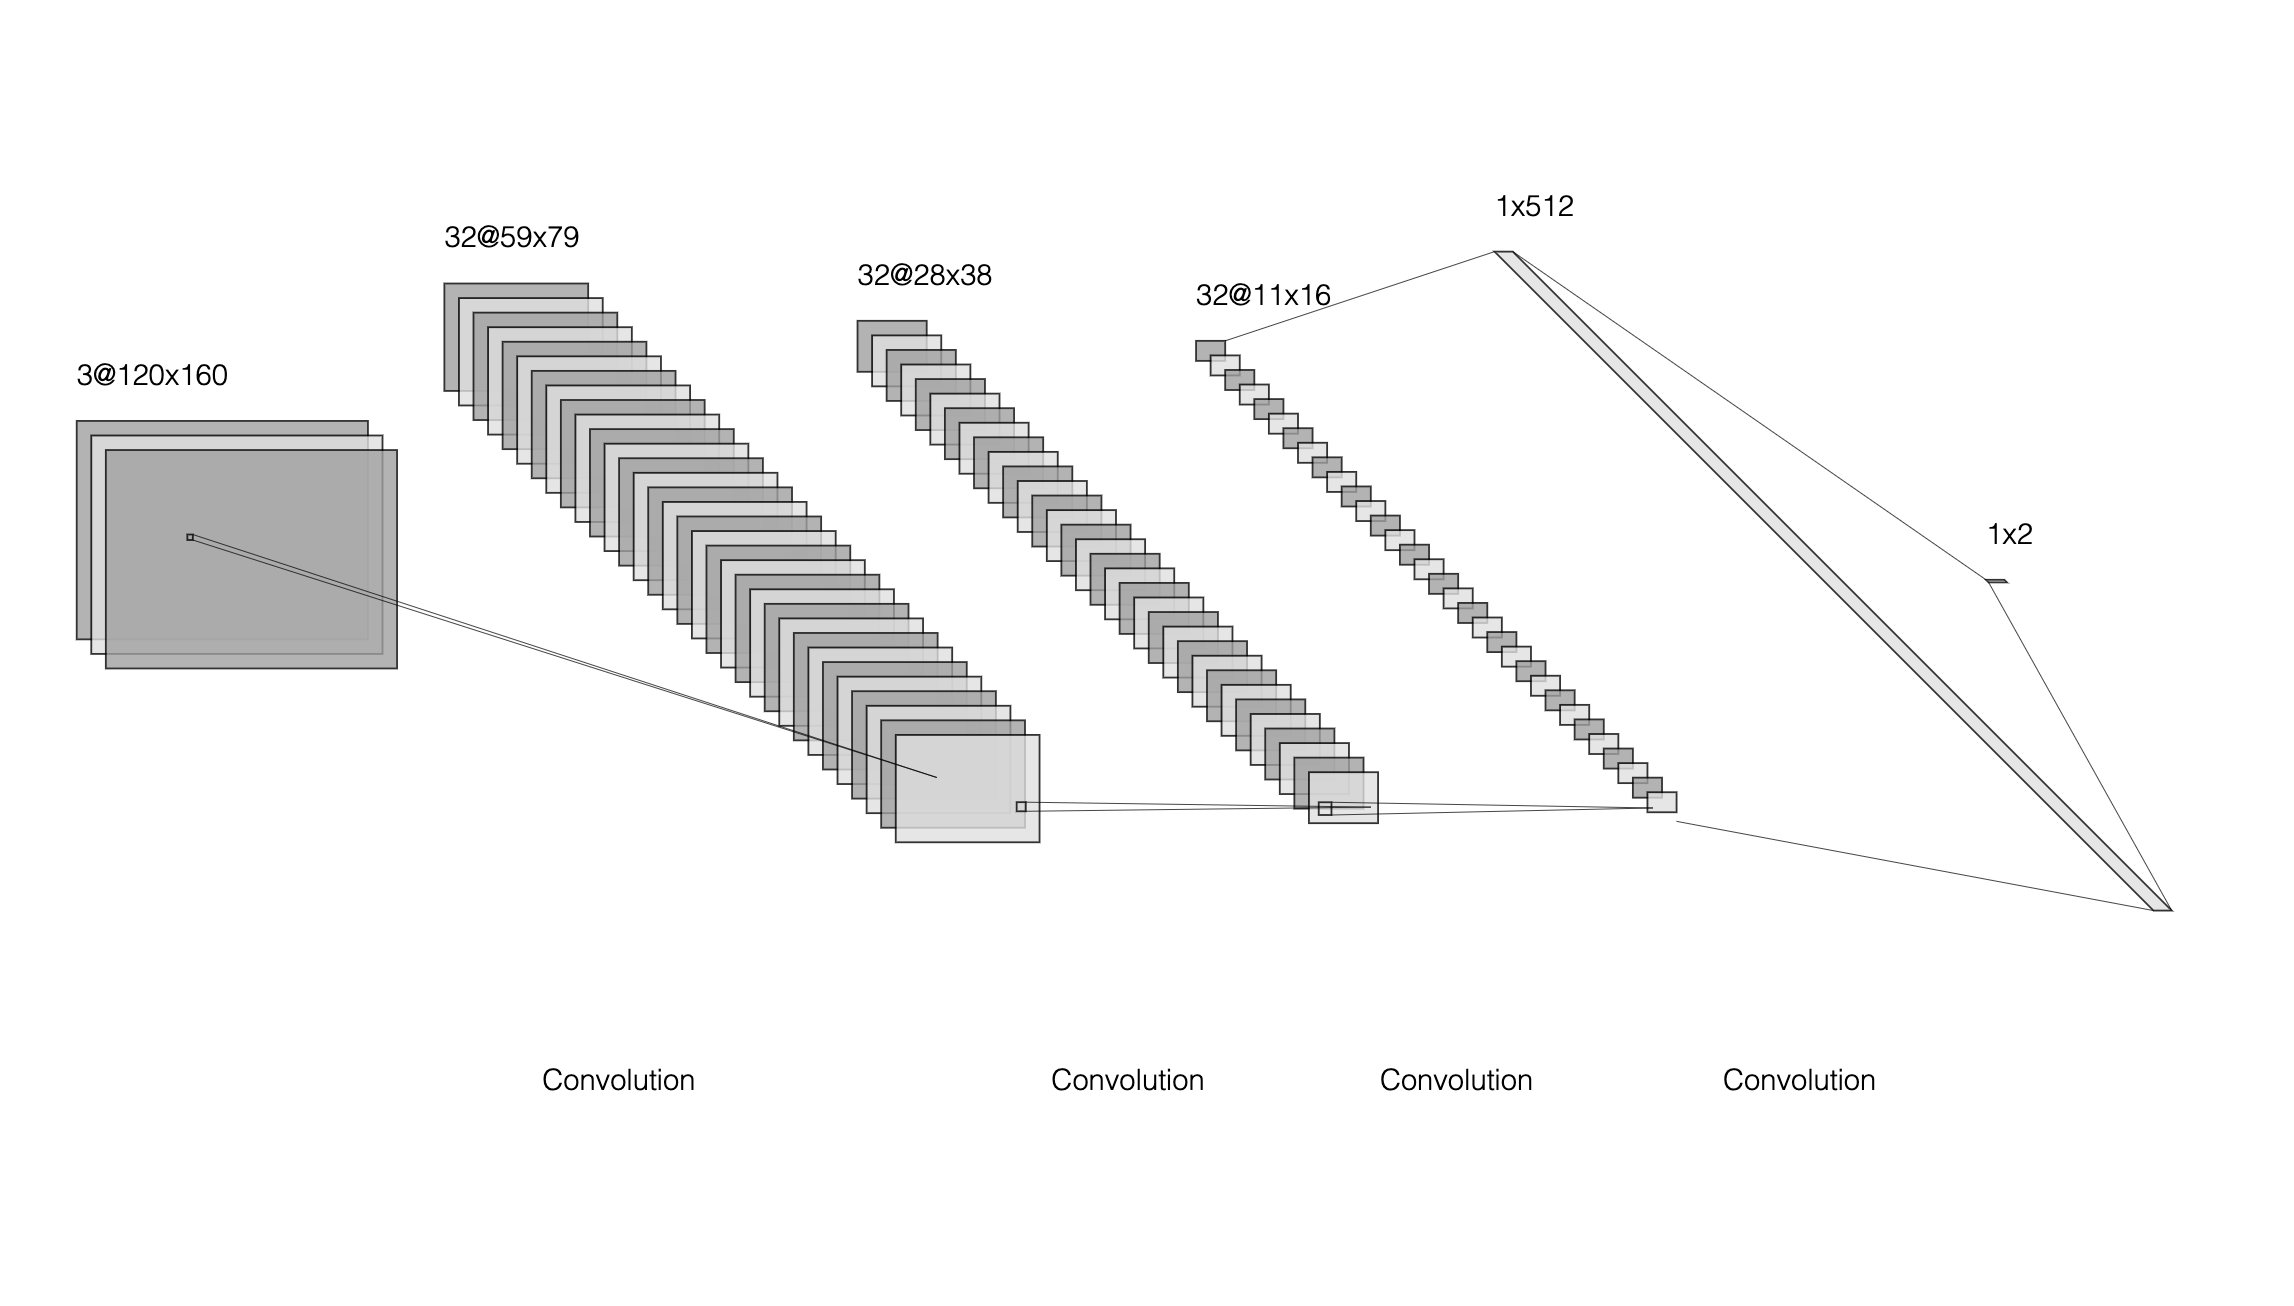
\includegraphics[scale=0.20]{neural_net.png}
  \caption{Neural Network Diagram}
\end{figure}
In this architecture, each convolutional block consists of a convolution, rectified linear unit, and
a batch normilization. The 4 convolutional blocks extract features from the AV camera while reducing
the state space of the image. Then information is then passed to the 2 fully connected layers to convert 
the states to the action space. 

\subsection{Learning}
The learning process used in this paper follows the process outlined in the deep active imitation
learning paradigm by \citet{deepImitation}. The process is as follows: (1) collecting demonstrations. 
(2) Supervised training of the neural network. (3) Active learning to refine the initially learned policy.
\subsubsection{Collecting Demonstrations}
Imitation learning requires expert behavior examples in order to train the model. For this paper, 
the expert examples were obtained from manually driving multiple laps of each test track. During 
the laps, the obvservation state and the action taken were recorded.
\subsubsection{Supervised Training}
Once recorded, the network is then trained on batched samples of the recorded observations and actions.
The loss function used was the cross entropy loss between the network action output and the 
expert action taken at that particular observation. 
\subsubsection{Dagger Re-Training}
After the supervised training has completed, the model is then run through the test tracks autonomously,
where the policy is continously refined using an L2 loss function. 

\section{Progress Thus Far} 
\label{sec:conclusion}

Thus far, I have set up the infrastructure to train the AV. The game code has been modified to 
generate various test and training tracks with random obstacles, and the code has been written to 
record the expert behaviors when driving manually through the simulator. The models and in the infrastructure
for the deep learning pipeline have also been created so that once the expert laps have been recorded,
training can begin to occur. 

%% Use plainnat to work nicely with natbib. 

\bibliographystyle{plainnat}
\bibliography{references}

\end{document}


